\label{sec:glossary}

In this section, our terminology is described, also with the general structure of work with translation memory.
% from which a design of common classes is inferred, later used both in US, GUI and Core. It also explains the terminology we use both in code and the documentation.

\subsection*{User}
Everyone, who logs into the system, is called \emph{User}. Each user of the TM has its own setting, authentication data etc., and can own multiple subtitle files which we call \emph{Documents}.

\subsection*{Document}
A \emph{document} is subtitle file, owned by a user. (This is not connected with files, that are used for building the corpus.) The documents contains information about \emph{media source} of the subtitle, and list of the subtitles \emph{chunks} which either have been already translated or are waiting for translation.

\subsection*{Media source}
\emph{Media source} is our name for specific movie or TV show episode. It contains the name of the movie, its release year and a set of tags describing the genre of the movie.

\subsection*{Chunk}
A \emph{chunk} is a piece of text, that is getting translated. As we will describe later, it doesn't have to be a complete sentence.

\subsection*{Surface form}
Every chunk has a \emph{surface form} -- that means the text, that is being translated. The surface form is without any non-textual information -- we store these in annotations.

\subsection*{Annotations}
Every chunk also has \emph{annotations} -- non-textual information, that might be used at some point, but are not sent to translation memory for querying. By that, we mean positions of named entities, original position of newlines and dialog marks ("-") -- none of these go into the translation memory core.

\subsection*{Timed chunk}
A \emph{timed chunk} is a chunk, that also have a time information and information about order, in which it appears in subtitle file.

\subsection*{Translation result}
The chunks are wrapped in to the \emph{Translation result} objects which contains the the timed chunk from the original subtitle file, a chunk produced by the user as a translation of the original chunk, a list of translation suggestions from translation memory.

\subsection*{Subtitle item}
To have a clear terminology, in this document, we will call \emph{subtitle item} the whole text, that has a time declaration in the video file and has a clear time information and is displayed in the video in a given time when playing. This differs from the \emph{timed chunk}, because we might split the subtitle item into more chunks and translate them differently.

Unfortunately, in the code itself, we call \emph{chunk} both the sentence, that is translated, and the whole subtitle item. This is an error on our part, created by not exactly defining all the terms beforehand and just using the term \emph{subtitle chunk} for everything.


\begin{figure}[h]
\begin{center}
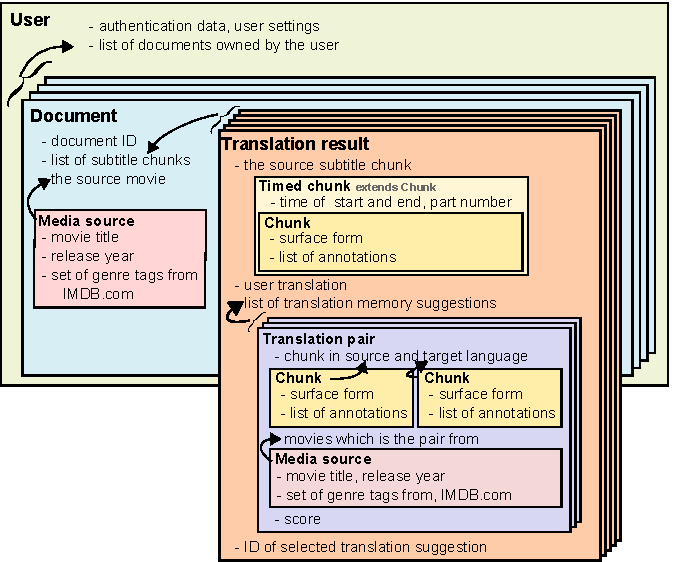
\includegraphics{figures/shared_classes.pdf}
\end{center}
\caption{Scheme of the application architecture.}\label{projectStructure:logical}
\end{figure}

%Deleting this, since we say the same stuff in the next section
%All mentioned characteristics are common for both US and GUI. Because all parts of the project are Java based we can use a set of shared classes. Despite the limitations of GWT, which implements only a subset of Java functionality, using a shared classes structure makes the whole project clearer. 
